\subsection{Diagrammi di sequenza}
\begin{figure}[hb]
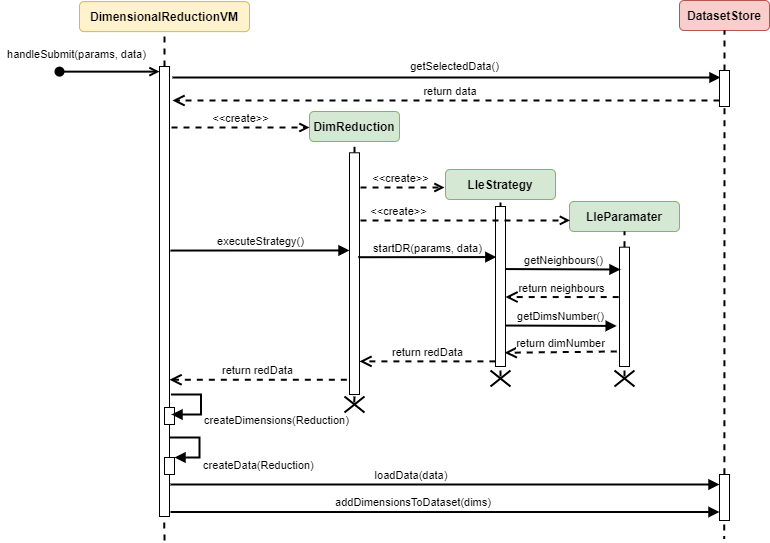
\includegraphics[width=16cm]{Images/Allegato Tecnico-Sequenza-DR}
\centering
\caption{Diagramma di sequenza che modella il processo di riduzione dimensionale con algoritmo LLE}
\end{figure}
Il diagramma di sequenza sopra riportato è cosi descritto:
\begin{enumerate}
	\item \textbf{DimensionalReductionVM}, che corrisponde al \textit{ViewModel} della parte di vista dedicata alla riduzione dimensionale, riceve l'algoritmo e i relativi valori dei parametri impostati dall'utente, prende i dati su cui eseguire la riduzione dal \textbf{DatasetStore} e crea il contesto, ossia \textbf{DimReduction};
	\item DimReduction si occupa di creare un'istanza della classe concreta dell'algoritmo scelto dall'utente (nell'esempio LLE, definito in \textbf{LLEStrategy}) e un'istanza della classe dei corrispettivi parametri (ossia \textbf{LLEParameter}), utilizzando i valori passatigli per settarne i vari attributi;
	\item Chiama poi \texttt{startDR()} sull'algoritmo, fornendo i dati e l'istanza della classe dei parametri. I valori di quest'ultimi vengono presi dall'algoritmo attraverso dei getter (nell'esempio \texttt{getNeighbours()} e \texttt{getDimensionsNumber()}) verso l'istanza di LLEParameter;
	\item \texttt{startDR()} a questo punto può eseguire la riduzione dimensionale utilizzando i metodi forniti dalla libreria Druid.js e ritornare un oggetto con dentro i nuovi dati e le nuove dimensioni;
	\item In DimensionalReductionVM vengono estrapolati i dati e le dimensioni dall'oggetto e caricate nel DatasetStore.
\end{enumerate}

\newpage
\begin{landscape}
\begin{figure}[hb]
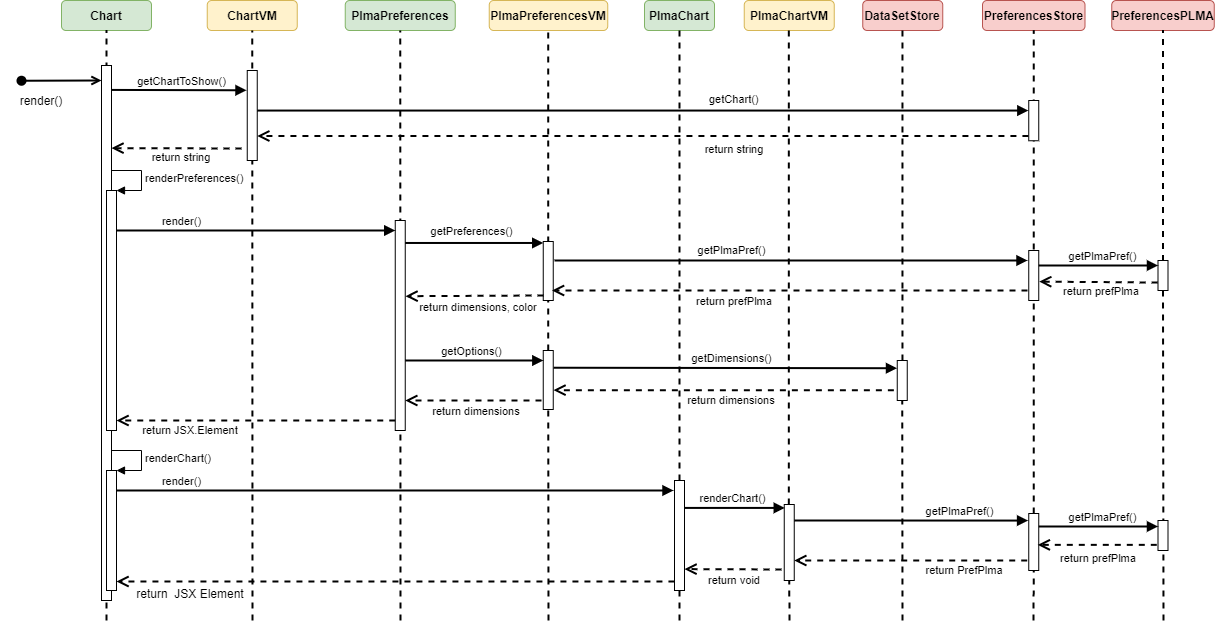
\includegraphics[width=\linewidth ,height=14cm]{Images/Allegato Tecnico-Sequenza-PLMApref}
\centering
\caption{Diagramma di sequenza che modella il processo di visualizzazione del grafico PLMA e del relativo box di preferenze}
\end{figure}
\end{landscape}
Il diagramma di sequenza sopra riportato è così descritto:
\begin{enumerate}[label=\textbf{\arabic*})]
	\item \textbf{Chart} è il componente React che renderizza la parte di vista contente il grafico e il relativo box di preferenze. Con \texttt{getChartToShow()} e \texttt{getChart()} di \textbf{ChartVM} (il corrispettivo \textit{ViewModel}) seleziona dal \textbf{PreferencesStore} la stringa che definisce quale box visualizzare (in questo esempio "PLMA");
	\item Sono quindi renderizzate le preferenze (\textbf{PlmaPreferences}), ossia la form utilizzabile dall'utente per modificare le caratteristiche di visualizzazione del PLMA. Inizialmente ogni suo campo input è vuoto e quindi non verrà visualizzato il grafico; 
	\item Ogni volta che l'utente modifica tale form avviene una rirenderizzazione del box delle preferenze e del grafico. Tale modifica comporta la chiamata al \textbf{PlmaPreferencesVM} (\textit{ViewModel} delle preferenze del PLMA) che si occupa di prelevare dai vari store (\textbf{PreferencesStore} e \textbf{DatasetStore}) le informazioni necessarie per cambiare in real-time la vista;
	\item È quindi renderizzato il PLMA (in \textbf{PLMAChart}) con le varie modifiche di visualizzazione impostate dall'utente.
\end{enumerate}

\newpage